%% COMP90083 Computational Modelling & Simulation
%% Assignment 2, final report. Affordable rental supply and displacement.
%% Plain-language edition of COMP90083_Project_2_Affordable_Rental_Proposal.tex (same content, rewritten prose).

\documentclass[10pt,a4paper]{article}

\usepackage[a4paper, margin=25mm]{geometry}
\usepackage{graphicx}
\usepackage{booktabs}
\usepackage{parskip}
\usepackage{microtype}
\usepackage{hyperref}
\usepackage{url}
\usepackage[numbers,sort&compress]{natbib}
\usepackage{caption}
\usepackage{amsmath}
\usepackage{amssymb}
\usepackage{array}
\newcolumntype{L}[1]{>{\raggedright\arraybackslash}p{#1}}
\usepackage{xcolor}
\usepackage{enumitem}
\usepackage[T1]{fontenc}
\usepackage[sfdefault]{FiraSans}
\usepackage{tikz}
\usetikzlibrary{arrows.meta}
\renewcommand*\oldstylenums[1]{{\firaoldstyle #1}}

\hypersetup{
    colorlinks = true,
    breaklinks = true,
    bookmarks  = true,
    linkcolor  = blue!60!black,
    citecolor  = blue!60!black,
    urlcolor   = blue!60!black
}

\newcommand{\todo}[1]{\textcolor{red!70!black}{\textbf{[TODO: #1]}}}
\newcommand{\note}[1]{{\color{blue!70!black}#1}}

\captionsetup{font=small, labelfont=bf}

% ---- Final report ---------------------------------------------------------
% Report only. The proposal version (submitted 20 September 2026) is kept in
% .revision_backups/. Build with:
%   latexmk -pdf COMP90083_Project_2_Affordable_Rental_Proposal_natural.tex
\renewcommand{\baselinestretch}{1.1}
% floats stay at the top of a page or on a float page, and never drift past the references
\renewcommand{\topfraction}{0.85}
\renewcommand{\textfraction}{0.15}
\renewcommand{\floatpagefraction}{0.7}
\usepackage{placeins}

\begin{document}

\begin{center}
    {\Large\bfseries Spatial Allocation of Affordable Rental Supply and Displacement in a Stylised Greater Melbourne Rental Market}\\[0.8em]
    {\large COMP90083 Computational Modelling \& Simulation}\\[0.4em]
    {\normalsize
        Ivan Ramos Sampe Immanuel \quad Student ID: 1795375\\[0.2em]
        Fella Ulandari \quad Student ID: 1697938}\\[0.4em]
    {\normalsize The University of Melbourne \quad Semester 2, 2026}\\[0.4em]
    {\normalsize Final Report\quad Word count: 3,298}
\end{center}

\noindent\rule{\textwidth}{0.4pt}

\section*{Introduction}

Housing in Greater Melbourne has become hard to afford, and lower-income renters bear most of the cost. Rental stress that lasts leads to arrears, forced moves, and sometimes involuntary displacement, a forced move after which the household cannot find anywhere to live. In 2016 Melbourne had about 70,000 lowest-quintile private-renter households and only 7,200 dwellings both affordable and available to them, and nine in ten paid unaffordable rent \citep{1}. Nationally the shortage for these renters was 255,000 dwellings in 2021, or 348,000 excluding affordable homes occupied by higher-income renters \citep{2}. Victoria's \$5.4 billion Big Housing Build aims to deliver more than 12,000 homes, 9,300 of them social housing, so where they go is a live question \citep{3}.

Housing economics ties supply constraints to prices \citep{4} and location to job matching \citep{5}, and spatial mismatch theory adds that distance from jobs cuts employment through commuting costs and weaker job search \citep{6,7}. In Melbourne rental stock affordable to lower-income workers grew mostly in outer areas in the decade to 2016 while shortages were sharpest in inner and middle suburbs, so lower-income workers end up stressed, commuting far, or both \citep{8}. Their workplaces are spread widely, so housing near their ten main job destinations would reach only about a third of Melbourne's lower-income renters with above-average commuting burdens \citep{9}. Concentrating lower-income households may also tip a neighbourhood past a threshold beyond which harms begin \citep{10}. Whether to concentrate or spread supply is open.

A forced move is not the same as choosing to move \citep{11}, and it raises a working renter's chance of later losing a job \citep{12}. In Australia more than a quarter of low-income renters' moves happen because the property was no longer available \citep{13}. 

New supply in accessible places can protect existing renters, but it may also draw in movers who compete with them (induced demand) and push local rents up (rent feedback). Been et al.\ largely reject such supply-sceptic arguments for market housing \citep{14}, but whether they hold for rationed affordable units remains open. A new unit also protects in two ways, a cheaper rent and a tenancy that is hard to end, and private renting offers little of the second \citep{13,15}.

Econometrics mainly judges allocations already tried, system dynamics hides household differences, and spatial microsimulation needs local data we lack. Agent-based models (ABMs) of housing avoid these limits, with households of different incomes searching under budget limits and prices emerging from local transactions \citep{16,17}. Gentrification models show lower-income residents displaced as rents or property values rise \citep{18,19}, in one case whenever housing costs pass an agent's budget \citep{20}, and a Greater Sydney model links local government areas in a graph rather than a grid \citep{21}. Equilibrium and structural models have compared where affordable housing goes, one favouring the suburbs in a two-zone city \citep{22} and another higher-opportunity neighbourhoods with better schools and jobs \citep{23}. We found no ABM that makes location the lever while holding the total fixed and separates a unit's discount from its security.

We built a stylised model of a Melbourne-like region and compared a no-new-supply baseline with three ways of placing the same new affordable dwellings, with displacement first and stress second. We expected concentration near jobs to protect lower-income renters unless induced demand and rent feedback ate into that, and secure tenure rather than the discount to carry most of the protection.

\section*{Research Question}

In a stylised Melbourne rental market, does concentrating a fixed number of new affordable rental dwellings near jobs prevent more involuntary displacement of lower-income renters than spreading them by need or evenly?


%%%%%%%%%%%%%%%%%%%%%%%%%%%%%%%%%%%%%%%%%%%%%%%%%%%%%%%%%%%%%%%%%%%%%%%%%%%%%
\section*{Model Description}
%%%%%%%%%%%%%%%%%%%%%%%%%%%%%%%%%%%%%%%%%%%%%%%%%%%%%%%%%%%%%%%%%%%%%%%%%%%%%

\subsection*{Overview}

\subsubsection*{Purpose}

This description follows the ODD protocol \citep{24}. The model tests whether where a fixed number of new affordable dwellings go changes involuntary displacement among lower-income renters, with stress as a secondary outcome, once households can move toward new supply and rents respond to demand. Its benchmark is an allocation calculator, under which every unit prevents one displacement, so 10 per cent supply would cut displacements per household by 0.100 under any strategy.

\subsubsection*{Entities, State Variables, and Scales}

Households are the only agents, 1,000 of them. Each keeps base and current income, tenure (market, affordable, unhoused), its neighbourhood, accessibility at $t=0$, rent paid, stress and displacement counters, and pre-drawn shock and termination tables. Neighbourhoods form the environment, a ring of 20 nodes in three accessibility tiers, an arc of six high ($a_j=1.0$), four medium (0.6) on each side, and an arc of six low (0.3) opposite, and a shortcut parameter adds random edges between non-adjacent nodes. Each neighbourhood keeps its stock, occupancy, rent, rent pressure, background demand, cost index, and applications. A tick is a quarter and a run is 40 quarters. Table~\ref{tab:interaction} gives sensing and interaction, and Table~\ref{tab:params} the symbols.

\begin{table}[tp]
\centering
\caption{Sensing and interaction between entities.}
\label{tab:interaction}
\small
\begin{tabular}{L{2.4cm}L{6.1cm}L{6.1cm}}
\toprule
 & \textbf{Household} & \textbf{Neighbourhood} \\
\midrule
\textbf{Household} &
Does not sense other households directly. Senses last quarter's queue (applicants per vacancy) at each sampled option. Interacts through matching. Applicants for the same unit compete, and a unit taken is gone for the rest that quarter. &
Senses rent, vacancies, and accessibility in its own neighbourhood and in $k-1$ sampled ones, affordable vacancies only at home, and with induced demand on, every neighbourhood holding an affordable vacancy, its market vacancies included. Interacts by applying, moving in, or being terminated. \\
\addlinespace
\textbf{Neighbourhood} &
Does not sense individual households. Aggregates occupants, last quarter's applicants (rent feedback on), and background demand into rent pressure, which raises the termination hazard for its tenants. &
Neighbourhoods do not interact with one another. Network distance between them enters only through household moving cost. \\
\bottomrule
\end{tabular}
\end{table}

\subsubsection*{Process Overview and Scheduling}

Each quarter, in order, incomes update, tenancies end, rents update, stress is classified \citep{25}, market tenants and the unhoused search and get matched (anyone unhoused for $s$ quarters is displaced), the quarter's tranche of supply lands under the strategy, and outputs are recorded. Figure~\ref{fig:flow} shows where the strategies differ.

\begin{figure}[t]
\centering
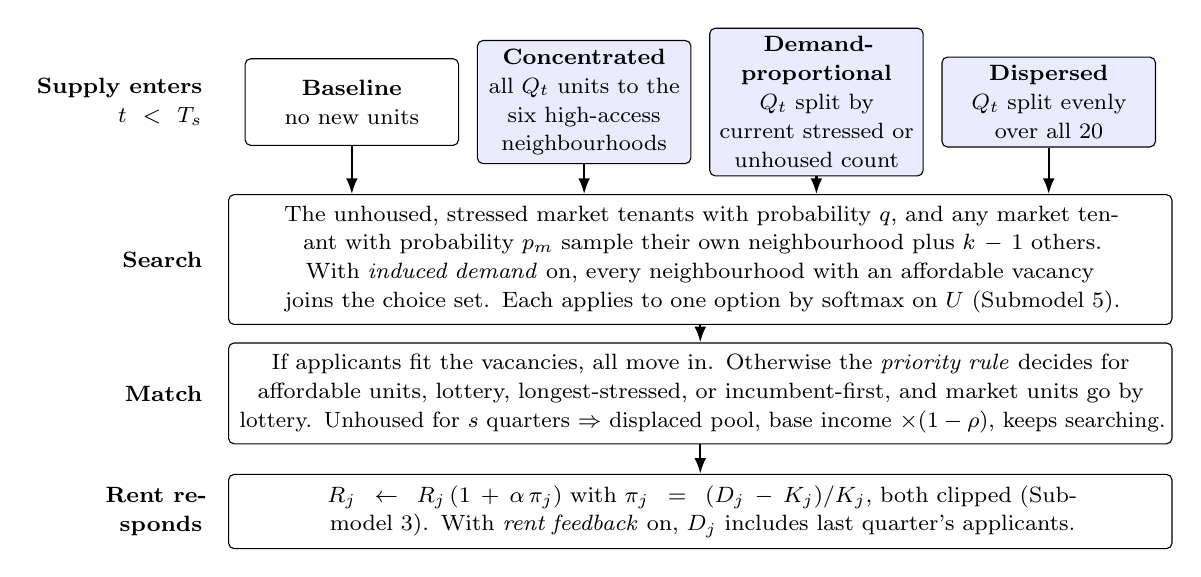
\begin{tikzpicture}[
  font=\footnotesize,
  box/.style={draw, rounded corners=2pt, align=center, text width=2.5cm, minimum height=1.1cm, inner sep=3pt},
  pol/.style={fill=blue!8},
  wide/.style={draw, rounded corners=2pt, align=center, text width=11.7cm, inner sep=4pt},
  lab/.style={font=\footnotesize\bfseries, align=right, text width=2.1cm},
  arr/.style={-{Latex[length=2mm]}, thick}
]
\node[lab] at (-1.5, 0) {Supply enters\\ $t<T_s$};
\node[box] (b1) at (1.45, 0) {\textbf{Baseline}\\ no new units};
\node[box, pol] (c1) at (4.4, 0) {\textbf{Concentrated}\\ all $Q_t$ units to the six high-access neighbourhoods};
\node[box, pol] (d1) at (7.35, 0) {\textbf{Demand-proportional}\\ $Q_t$ split by current stressed or unhoused count};
\node[box, pol] (e1) at (10.3, 0) {\textbf{Dispersed}\\ $Q_t$ split evenly over all 20};
\node[lab] at (-1.5, -2.0) {Search};
\node[wide] (w2) at (5.875, -2.0) {The unhoused, stressed market tenants with probability $q$, and any market tenant with probability $p_m$ sample their own neighbourhood plus $k-1$ others. With \emph{induced demand} on, every neighbourhood with an affordable vacancy joins the choice set. Each applies to one option by softmax on $U$ (Submodel 5).};
\node[lab] at (-1.5, -3.7) {Match};
\node[wide] (w3) at (5.875, -3.7) {If applicants fit the vacancies, all move in. Otherwise the \emph{priority rule} decides for affordable units, lottery, longest-stressed, or incumbent-first, and market units go by lottery. Unhoused for $s$ quarters $\Rightarrow$ displaced pool, base income $\times(1-\rho)$, keeps searching.};
\node[lab] at (-1.5, -5.2) {Rent responds};
\node[wide] (w4) at (5.875, -5.2) {$R_j \leftarrow R_j\,(1+\alpha\,\pi_j)$ with $\pi_j=(D_j-K_j)/K_j$, both clipped (Submodel 3). With \emph{rent feedback} on, $D_j$ includes last quarter's applicants.};
\foreach \n in {b1,c1,d1,e1} \draw[arr] (\n.south) -- (\n.south |- w2.north);
\draw[arr] (w2) -- (w3);
\draw[arr] (w3) -- (w4);
\end{tikzpicture}
\caption{Household movement and matching under each allocation strategy. Shaded boxes are the policy conditions and the three lower rows are shared. Induced demand and rent feedback are two of the four stage 3 switches. Units land after matching, and rent responds to this quarter's applicants at the start of the next quarter. Symbols are defined in Table~\ref{tab:params} and Submodels 1 to 6.}
\label{fig:flow}
\end{figure}

\subsection*{Design Concepts}

\subsubsection*{Basic Principles}

Three ideas drive the design, bounded-rational search \citep{26} under a budget, spatial mismatch \citep{6,7}, and matching in a rationed market, where one household winning a unit moves a rival closer to displacement. We treat the search rule as a theory to test \citep{27,28}, with search-rule random as the null, then cheapest, then utility. We use a network of neighbourhoods rather than a grid of house patches because the policy lever, rents, queues, and termination pressure act at neighbourhood level, and moving cost depends on how far apart suburbs sit, which a graph represents directly, as in \citep{21}. House patches would add state no rule reads, and a graph lets robustness runs add shortcuts. A household's stress makes it search but does not raise its own termination risk, and accessibility enters preferences, not income. We left out landlord agents for build time and added demand-proportional allocation because planners use it. An equation-based version (expected flows, no lottery) runs beside the agent model.

\subsubsection*{Adaptation, Objectives, Learning, Prediction, Sensing, Interaction, Collectives}

Households adapt by searching when terminated or stressed, choosing by the softmax utility of Submodel 5. Learning and prediction are absent, since households do not remember outcomes or forecast rents. Collectives are absent, as households form no groups.

\subsubsection*{Emergence}

We expected displacement differences from the calculator's one per unit and drift away from jobs to emerge, and neither is coded. The gap between the full model and the switched-off or equation-based runs is the emergent effect.

\subsubsection*{Stochasticity}

Randomness enters through incomes, placement, shortcuts, the shock and termination tables, search, and matching. Draws that do not depend on the strategy come first, so runs sharing a seed share shocks, and strategies are compared within seed.

\subsubsection*{Observation}

Each quarter we record displacements per household, stress prevalence, access lost, rent increase by tier, units delivered, and the forced-move share, overall and by place and income. Pairing displacement with accessibility lost mirrors IFC Performance Standard 5 \citep{29}.

\subsection*{Details}

\subsubsection*{Initialisation}

Neighbourhoods start from Table~\ref{tab:params} with no affordable capacity, households draw base incomes from $U(0.6,1.0)$ and are placed as market tenants in proportion to vacancies, and the number of new dwellings is $N=\mathrm{round}(\sigma n)$, with the remaining initial state in Table~\ref{tab:details}.

\subsubsection*{Input Data}

There is no time-series input, and every parameter is from the literature, calibrated, or a stated assumption (Table~\ref{tab:params}).

\begin{table}[tp]
\centering
\caption{Model parameters, with each one's variable name in the NetLogo model. In the source column L means literature or regulation, C calibrated to patterns P1 to P4 (Methods), A assumed, and D a design choice. Rents and incomes are shares of a reference quarterly income.}
\label{tab:params}
\footnotesize
\begin{tabular}{L{3.5cm}L{3.5cm}L{1.6cm}L{2.3cm}L{3.0cm}}
\toprule
\textbf{Parameter} & \textbf{NetLogo name} & \textbf{Symbol} & \textbf{Value} & \textbf{Source} \\
\midrule
Households & \texttt{\scriptsize n-households} & $n$ & 1,000 & A (scale) \\
Neighbourhoods, tiers high/medium/low & \scriptsize fixed in setup & & 20, 6/8/6 & A \\
Shortcut edges on the ring & \texttt{\scriptsize n-shortcuts} & & 0 (robustness runs 3, 8) & A \\
Affordability screen on new tenancies, landlord screening & \texttt{\scriptsize max-rent-to-income,\allowbreak{} landlord-screening?} & & 0.5 of income, off & A, looser than the 30\% affordability benchmark \citep{25}, P4 holds without this screen. \\
Market stock per neighbourhood, high/medium/low & \texttt{\scriptsize stock-high/mid/low} & $M_j$ & 40/55/60 & A (1,040 total) \\
Initial rent, high/medium/low & \texttt{\scriptsize rent-high/mid/low} & $R_{j,0}$ & 0.38/0.31/0.25 & C (P1 fails at $\pm$10\%) \\
Base income range & \texttt{\scriptsize income-min,\allowbreak{} income-max} & $\bar y_i$ & $U(0.6,1.0)$ & C (P1) upper bound, A lower \\
Background demand, share of market stock, high/medium/low & \texttt{\scriptsize non-target-frac-\allowbreak high/mid/low} & $b_j$ & 0.30/0.15/0 & C (P1, P3) \\
Rent responsiveness & \texttt{\scriptsize alpha} & $\alpha$ & 0.03 & C (P3) \\
Income growth per quarter & \texttt{\scriptsize income-growth} & $g$ & 0.01 & C (P1) \\
Shock probability, size, duration & \texttt{\scriptsize p-income-shock,\allowbreak{} income-shock-size,\allowbreak{} shock-duration} & $p,\ \delta$ & 0.05, 0.20, 4 quarters & A \\
Termination hazard, pressure coefficient & \texttt{\scriptsize termination-hazard-base,\allowbreak{} termination-hazard-coef} & $h_0,\ \kappa$ & 0.006, 2 & C (P2), A (P1--P4 hold for 1--3) \\
Stress threshold & \texttt{\scriptsize stress-threshold} & $\theta$ & 0.30 & L \citep{25} \\
Search probability when stressed & \texttt{\scriptsize search-prob} & $q$ & 0.25 & A (P1--P4 hold for 0.15--0.35) \\
Move probability unrelated to stress & \texttt{\scriptsize bg-target-move-prob} & $p_m$ & 0.15 & C (P2) \\
Higher-income renters take and hold market vacancies & \texttt{\scriptsize non-target-competition?} & & on, share $b_j$ & C (P3), extends \citep{2} \\
Neighbourhoods sampled & \texttt{\scriptsize n-search-towns} & $k$ & 4 & A \\
Search period before displacement & \texttt{\scriptsize s-search-period} & $s$ & 2 quarters & A \\
Income penalty on displacement & \texttt{\scriptsize income-penalty} & $\rho$ & 0.15 & A, direction from lay-off evidence \citep{12} \\
Utility weights rent/access/queue, moving cost, noise & \texttt{\scriptsize weight-rent,\allowbreak{} weight-access,\allowbreak{} weight-queue,\allowbreak{} moving-cost,\allowbreak{} choice-noise} & $w_r$, $w_a$, $w_q$, $m$, $\tau$ & 5, 1, 1, 0.3, 0.3 & A \\
Affordable rent as share of market rent (1 with the discount switch off), or of income & \texttt{\scriptsize affordable-rent-ratio,\allowbreak{} rent-discount?,\allowbreak{} income-rent-share} & $\lambda$, $\eta$ & 0.75, 0.25 & A, set from Victorian performance standards \citep{30} \\
Affordable tenancy security & \texttt{\scriptsize secure-tenure?} & & secure & D, from Victorian performance standards \citep{30}, approximating stronger tenure security \\
New supply as share of households, window & \texttt{\scriptsize govt-homes,\allowbreak{} govt-homes-build-time} & $\sigma,\ T_s$ & 10\%, 8 quarters & D \\
Budget view, cost index high/medium/low & \texttt{\scriptsize fixed-budget?,\allowbreak{} cost-high/mid/low} & $c_j$ & fixed supply, 1.6/1.0/0.7 & D, A \\
Priority rule & \texttt{\scriptsize priority-rule} & & lottery & D \\
Search rule, induced demand, rent feedback, discount, rent rule & \texttt{\scriptsize search-rule,\allowbreak{} induced-demand?,\allowbreak{} rent-feedback?,\allowbreak{} rent-discount?,\allowbreak{} affordable-rent-rule} & & utility, on, on, on, market share & D \\
Run length, seeds per condition & \scriptsize BehaviorSpace time limit, \texttt{seed} & & 40 quarters, 50 (30 or 10 for checks) & D \\
\bottomrule
\end{tabular}
\end{table}

\begin{table}[tp]
\centering
\caption{Rules a reimplementation needs beyond Submodels 1 to 6, as coded in the NetLogo model.}
\label{tab:details}
\footnotesize
\begin{tabular}{L{3.0cm}L{11.5cm}}
\toprule
\textbf{Rule} & \textbf{Detail} \\
\midrule
Initial state & No dwellings held by higher-income renters and zero pressure. Households are placed one at a time in proportion to remaining vacancies, then the random tables are drawn and stress is classified, so the stressed-quarters counter starts at 1 for households stressed at setup. Households also keep their initial income, for income thirds, and an ever-displaced flag. \\
Layout & Neighbourhood ids 0 to 19 run round the ring (degree 2, clustering 0, characteristic path length 5.26). High tier 7 to 12, medium 3 to 6 and 13 to 16, low 0 to 2 and 17 to 19. Shortcuts join random non-adjacent pairs. \\
Choice set & A market tenant has no market option in its own neighbourhood. Induced demand adds every neighbourhood holding an affordable vacancy, with both its affordable and its market vacancies. Affordable tenants never search. \\
Matching order & All searchers choose first, against the vacancies at the start of matching. Neighbourhoods are then matched in random order, and within each one affordable units before market units. A mover's old market unit is freed at once and can be filled by a neighbourhood matched later. \\
Higher-income renters & Each quarter, at its market step and whether or not anyone applied, each neighbourhood loses each current market vacancy to them with probability $b_j$. Units they hold are released at rate $h_0$. \\
Screens & The affordability screen uses current income and covers affordable options too. The 0.98 rent rule of Submodel 5 applies only to stressed market tenants not also drawn as $p_m$ movers. With no option left, no application is made. Landlord screening (off) would put market applicants never displaced first when units are oversubscribed. \\
Priority rules & Lottery draws winners at random. Longest-stressed takes the applicants with the most consecutive stressed quarters, ties at random. Incumbent-first takes applicants whose current or last dwelling is in $j$ first, the rest by lottery. Market vacancies are always a lottery. \\
Search theories & \texttt{search-rule} utility uses the softmax of Submodel 5, random weights every option equally, and cheapest takes the lowest-rent option, ties at random. \\
Displacement & The unhoused counter rises after matching, the termination quarter included. Rehousing resets it, and a later termination can displace the household again, with a further cut of $\rho$. In the leave reversal displaced households leave instead. \\
Income shocks & A shock drawn during an active shock is ignored. \\
Supply rounding & Each neighbourhood gets the floor of its amount, and the remaining $\mathrm{round}(\sum_j\text{amount}_j)$ minus the floors go to the largest remainders, so under a fixed budget the total can differ from $Q_t$. Remainder ties go to the neighbourhood with the fewest affordable units, then the lowest id. Halves round up. If every weight is zero, weights are equal. Demand-proportional weights use stress as classified at step 4 of the quarter and dwellings after matching. \\
Income-share rent & An affordable tenant pays $\eta\,y_{i,t}$ whatever the discount switch, and this rent enters the screen and the utility. \\
Metrics & $E$ (\texttt{displaced-share}) counts entries to the displaced pool per household. \texttt{forced-move-share} is terminations over terminations plus moves by market tenants. \texttt{access-lost} is $a_j$ at $t=0$ minus the current $a_j$, which is taken as 0 for the unhoused. \texttt{mean-stress-duration} (monitor ``mean stress quarters'') is the mean current run of stressed quarters among stressed households. First-year stress is the mean of \texttt{stress-prevalence} over quarters 1 to 4. \texttt{rent-increase-high}, \texttt{-mid} and \texttt{-low} are rent over initial rent by tier (the model's plot ``Rent Increase by Tier''). \\
Equation-based version & Each neighbourhood holds expected numbers of market tenants $H_j$, affordable tenants, unhoused $W_j$, displaced, and higher-income renters. Terminations and rents follow Submodels 2 and 3 as expected flows. The stressed share of market tenants is $f_j=\mathrm{clip}\big((R_j/\theta-0.6(1+g)^t)/(0.4(1+g)^t),0,1\big)$, for incomes uniform on $[0.6,1.0](1+g)^t$ with no shocks and no income cut. Searchers are the unhoused and displaced, $q f_jH_j$ stressed movers limited to options below 0.98 of $R_j$, and $p_mH_j$ other movers, who choose by the softmax at the mean income over every neighbourhood, with affordable options as in Submodel 5 and no affordability screen. Higher-income renters take $b_j$ of free market capacity and leave at rate $h_0$. Placements are capped by vacancies and shared pro rata between the unhoused and voluntary movers, and the unhoused enter the displaced pool at rate $1/s$ a quarter. Demand-proportional weights are $f_jH_j+W_j$. \\
\bottomrule
\end{tabular}
\end{table}


\subsubsection*{Submodels}

Household $i$, neighbourhood $j$, quarter $t$. $\mathrm{clip}(x,l,u)$ bounds $x$ to $[l,u]$. Table~\ref{tab:details} gives the remaining rules a reimplementation needs.

\textbf{1. Income.} $\bar y_{i,t}=\bar y_{i,t-1}(1+g)$, cut by $\rho$ at each displacement, and $y_{i,t}=\bar y_{i,t}(1-\delta)$ in the quarter of a shock, drawn with probability $p$, and the three after it, and $\bar y_{i,t}$ otherwise.

\textbf{2. Termination.} A market tenancy ends when the pre-drawn uniform $u_{i,t}<h_0\,(1+\kappa\,\max(0,\pi_{j,t-1}))$. Affordable tenancies are exempt unless the security switch is off.

\textbf{3. Rent.}
\begin{equation}
\pi_{j,t}=\mathrm{clip}\!\left(\frac{D_{j,t}-K_{j,t}}{K_{j,t}},-0.5,0.5\right),\qquad
R_{j,t}=\mathrm{clip}\!\big(R_{j,t-1}(1+\alpha\,\pi_{j,t}),\,0.5R_{j,0},\,3R_{j,0}\big),
\end{equation}
where $D$ counts occupied units, those held by higher-income renters included, last quarter's applicants (rent feedback on), and background demand $B_j=b_jM_j$, and $K$ is market stock $M_j$ plus affordable capacity.

\textbf{4. Stress.} Household $i$ is stressed when $r_{i,t}/y_{i,t}>\theta$, with $r=R_j$ for market tenants and $\lambda R_j$ for affordable tenants ($\lambda=1$ with the discount off), or $\eta\,y_{i,t}$ under the income-share rule. The unhoused count as stressed.

\textbf{5. Search and matching.} Searchers are the unhoused, stressed market tenants with probability $q$, and any market tenant with probability $p_m$. The choice set is the household's own (or last) neighbourhood and $k-1$ others drawn without replacement, with affordable vacancies visible only at home unless induced demand adds every neighbourhood holding one. An option is a neighbourhood and unit type with a vacancy, excluding a market tenant's home market units, with utility
\begin{equation}
U_{ij}=-w_r\frac{r_j}{y_{i,t}}+w_a a_j-m\Big(1+\frac{d_{ij}}{10}\Big)\mathbb{1}[j\neq \mathrm{home}_i]-w_q\ln\!\Big(1+\frac{A_j}{\max(1,V_j)}\Big),
\end{equation}
with $d_{ij}$ the network distance and $r_j$, $A_j$, and $V_j$ the option's rent, last quarter's applicants, and vacancies. Options above the affordability screen, 0.5 of current income, are dropped, and stressed market tenants keep only options below 0.98 of their rent. One application goes in with probability $\propto\exp(U_{ij}/\tau)$. Higher-income renters first take and hold each market vacancy with probability $b_j$, the rest go by lottery, and affordable units by the priority rule. After $s$ quarters unhoused a household is displaced, its base income is cut by $\rho$, and it keeps searching.

\textbf{6. Supply.} For $t<T_s$ the tranche is $Q_t=\mathrm{round}(N(t+1)/T_s)-\mathrm{round}(Nt/T_s)$, shared in proportion to $\omega_j=\mathbb{1}[\text{tier}_j=\text{high}]$ (concentrated), 1 (dispersed), or the count of stressed or unhoused households whose current or last dwelling is in $j$ (demand-proportional), rounded by largest remainder. Under a fixed budget neighbourhood $j$ gets $Q_t\omega_j/(c_j\sum_l\omega_l)$ dwellings before rounding.


%%%%%%%%%%%%%%%%%%%%%%%%%%%%%%%%%%%%%%%%%%%%%%%%%%%%%%%%%%%%%%%%%%%%%%%%%%%%%
\section*{Methods}
%%%%%%%%%%%%%%%%%%%%%%%%%%%%%%%%%%%%%%%%%%%%%%%%%%%%%%%%%%%%%%%%%%%%%%%%%%%%%

\textbf{Strategies and stages.} We compare a baseline and three ways of allocating the same $N$ dwellings in three stages (Table~\ref{tab:levels}). Stage 1 tests whether the ranking depends on quantity, window, or priority rule, after which the lottery is kept. Stage 2 answers the research question at every supply level, then under a fixed budget, where costlier tiers yield fewer dwellings. Stage 3 asks why, switching mechanisms off and crossing security, the discount, and the rent rule, and two diagnostics trace timing and induced demand.

\begin{table}[tp]
\centering
\caption{Experiments. Reference settings are in bold and every other setting is at its value in Table~\ref{tab:params}. Factors move one at a time from the reference unless crossed ($\times$), and every run lasts 40 quarters. The three priority rules differ by at most 0.003 in mean displacement, every paired interval includes zero, and every strategy keeps the lottery.}
\label{tab:levels}
\small
\begin{tabular}{L{3.0cm}L{7.3cm}L{2.5cm}L{1.4cm}}
\toprule
\textbf{Experiment} & \textbf{Factors and levels} & \textbf{Conditions} & \textbf{Seeds} \\
\midrule
Pilot grids 1 to 4 & three to six calibration parameters each & baseline & 1 to 10 \\
Final grid & \texttt{bg-target-move-prob} 0.10 to 0.18, \texttt{termination-hazard-base} 0.005 to 0.008, \texttt{non-target-frac-mid} 0.125 to 0.20, 144 sets & baseline & 1 to 50 \\
Unswept checks & \texttt{rent-high}, \texttt{-mid}, \texttt{-low} $\pm$10\%, \texttt{termination-hazard-coef} 1, 2, 3, \texttt{search-prob} 0.15, 0.25, 0.35 & baseline & 1 to 10 \\
Screening check & \texttt{max-rent-to-income} 0.5 or 1 $\times$ \texttt{landlord-screening?} $\times$ \texttt{non-target-competition?} & all four & 1 to 10 \\
Theory test & \texttt{search-rule} random, cheapest, \textbf{utility} & all four & 1 to 10, rerun with 1 to 50 for the ranking \\
Stage 1 & \texttt{govt-homes} 5, \textbf{10}, 15, 20, 30 (\% of households), \texttt{govt-homes-build-time} 1, 4, \textbf{8}, 16, 24, \texttt{priority-rule} \textbf{lottery}, longest-stressed, incumbent-first & three strategies & 1 to 50 \\
Window diagnostic & \texttt{govt-homes-build-time} 1, 8, 24 $\times$ \texttt{induced-demand?} & three strategies & 1 to 50 \\
Stage 2 & \texttt{govt-homes} 5 to 30, \texttt{mean-field?} \textbf{false} or true, then \texttt{fixed-budget?} true with \texttt{cost-high/mid/low} 1.6/1.0/0.7 & all four & 1 to 50 \\
Stage 3, mechanisms & \texttt{induced-demand?} $\times$ \texttt{rent-feedback?}, \textbf{true} or false & all four & 1 to 50 \\
Stage 3, unit & \texttt{secure-tenure?} $\times$ \texttt{rent-discount?}, \textbf{true} or false, $\times$ \texttt{affordable-rent-rule} \textbf{market-share} or income-share & all four & 1 to 50 \\
Induced-demand diagnostic & \texttt{induced-demand?} & three strategies & 1 to 30 \\
Sensitivity & 16 parameters $\pm$15\% or one step (\texttt{n-search-towns}, \texttt{s-search-period}), \texttt{cost-high} with \texttt{fixed-budget?} true & all four & 1 to 30 \\
Robustness & \texttt{termination-hazard-base} $\pm$15\%, another passing set, \texttt{displaced-leave?} true, no background demand, \texttt{n-shortcuts} 3 or 8 & all four & 1 to 30 or 1 to 50 \\
\bottomrule
\end{tabular}
\end{table}

\textbf{Metrics.} With $n$ households and $T=40$ the key metric is displacements per household,
\begin{equation}
E=\frac{1}{n}\sum_{i=1}^{n}\#\{t\le T : i \text{ entered the displaced pool at } t\},
\end{equation}
where a displacement is a forced move \citep{11} followed by $s$ quarters without a home, so a household rehoused and displaced again counts twice. A strategy's gain is its paired reduction in $E$ against the baseline. Counting households instead lowers values by 0.014 to 0.017 at 10 per cent supply and leaves the ranking unchanged. Displacement answers the research question, so every experiment is designed and ranked on $E$, and stress, rents, and accessibility are secondary outcomes used to explain it.

\textbf{Calibration.} We fit the baseline to four ranked patterns at four levels, each with a matching criterion (Table~\ref{tab:patterns}), in the pattern-oriented way \citep{27,28}. All four must hold at once, none may be hard-wired, and a set must stay inside the saturation band, $E$ between 0.20 and 0.60 and stress between 0.40 and 0.90 at quarter 40. Four pilot grids of ten seeds follow the ranking, and each failure pointed to a process we added (Table~\ref{tab:patterns}). A final grid of 144 sets with 50 seeds tests whether the patterns pin a point. Unswept parameters move one at a time, and the calibrated set is rerun under the three search theories.

\begin{table}[tp]
\centering
\caption{Calibration patterns, with the calibrated baseline over 50 seeds (values with the affordability screen off come from the ten-seed screening check). \texttt{access-lost} counts the unhoused as having no access, so ever-displaced households still unhoused at quarter 40 add to the P4 gap mechanically. The pilot failures pointed to the processes added. P2 needed moves unrelated to stress, and P3 higher-income renters holding high- and medium-tier vacancies, extending the competition for low-rent stock in \citep{2}. For P4 we put two candidates behind switches, landlord screening \citep{31} and an affordability screen on new tenancies \citep{13}.}
\label{tab:patterns}
\small
\begin{tabular}{L{2.0cm}L{3.1cm}L{1.0cm}L{3.0cm}L{1.95cm}L{2.0cm}}
\toprule
\textbf{Pattern (rank, level)} & \textbf{Stylised fact} & \textbf{Source} & \textbf{Matching criterion} & \textbf{Parameters fitted} & \textbf{Calibrated baseline} \\
\midrule
P1 Stress prevalence (1, population) & About 90 per cent of lowest-quintile private renters in Melbourne pay unaffordable rent & \citep{1} & \texttt{stress-prevalence} over quarters 1 to 4 between 0.85 and 0.95, and within the saturation band at quarter 40 & $\bar y_i$ range, $g$, $R_{j,0}$, $b_j$ & 0.87 first year, 0.87 and $E=0.28$ at quarter 40 \\
P2 Forced-move share (2, individual move) & About 28 per cent of low-income renters' moves occur because the property was no longer available & \citep{13} & \texttt{forced-move-share} between 0.20 and 0.35 & $h_0$, $p_m$ & 0.31 \\
P3 Rent gradient (3, neighbourhood) & Rents are highest in inner and middle suburbs, where shortages were sharpest in 2016 & \citep{1,8} & Rent Increase by Tier at quarter 40 ordered \texttt{rent-increase-high} $>$ \texttt{-mid} $>$ \texttt{-low}, so the gradient steepens & $\alpha$, $b_j$ by tier & 1.55, 1.45, 1.38 \\
P4 Displacement outcome (4, individual outcome) & Evidence from the United States indicates that forced movers relocate to poorer and higher-crime neighbourhoods than comparable voluntary movers. We use this as a stylised displacement pattern rather than a Melbourne-specific estimate & \citep{11} & \texttt{access-lost-}\allowbreak\texttt{displaced} greater than \texttt{access-lost-}\allowbreak\texttt{not-displaced} & none, checked not fitted & 0.34 against 0.04 (screen off 0.28 against 0.06) \\
\bottomrule
\end{tabular}
\end{table}

\textbf{Sensitivity.} Sixteen parameters move $\pm15$ per cent or one step under the baseline and each strategy at the reference settings, with seeds 1 to 30, and
\begin{equation}
\bar S=\tfrac{1}{2}\big(|S^{+}|+|S^{-}|\big),\qquad
S^{\pm}=\frac{1}{30}\sum_{e=1}^{30}\frac{E^{\pm}_e-E^{0}_e}{\Delta^{\pm}\,\bar E^{0}},
\end{equation}
with $E_e$ the value for seed $e$, $\bar E^{0}$ the reference mean, and $\Delta^{\pm}$ the parameter's relative shift, is reported for each parameter and condition. $\bar S$ carries no interval, so we also test the ranking in every setting.

\textbf{Parametrisation and assumptions.} The 30 per cent stress threshold is the rent test of the 30/40 convention \citep{25}, and every modelled household counts as lower-income. Displaced households lose 15 per cent of base income, since a forced move raises a working renter's chance of being laid off by 11 to 22 percentage points \citep{12}, and in the model a lower income narrows the options the affordability screen allows, making re-entry harder. The size is assumed, but $E$ barely responds to it ($\bar S$ at most 0.12). The cut is permanent and compounds on a repeat displacement, a simplification of a raised risk of job loss. The population is closed, accessibility is fixed, stress is binary, and there are no landlord agents.

\textbf{Protocol.} Development and tests are recorded in the model guide, README, and Info tab, short of full TRACE \citep{32}, and the search-theory ladder answers ODD\,+\,D's theory questions \citep{33}. Runs use NetLogo 7.0.4 BehaviorSpace with the seeds in Table~\ref{tab:levels}, paired by the pre-drawn tables. Effects are within-seed paired differences with 95 per cent percentile bootstrap intervals over seeds, from 2,000 resamples.

\textbf{Run length.} Because $E$ accumulates and never settles, our criterion is a stable ranking, and forty quarters meets it. From quarter 8 the baseline adds new displacements at a steady rate of about 0.0075 per household per quarter, concentration is the lowest strategy from quarter 2, and its lead over the best rival holds at 0.010 to 0.012 from quarter 12, so longer runs should raise every $E$ without changing the ranking. Units delivered after quarter 16 protect for under 24 quarters, so results for the 24-quarter window depend on the horizon.


%%%%%%%%%%%%%%%%%%%%%%%%%%%%%%%%%%%%%%%%%%%%%%%%%%%%%%%%%%%%%%%%%%%%%%%%%%%%%
\section*{Results}
%%%%%%%%%%%%%%%%%%%%%%%%%%%%%%%%%%%%%%%%%%%%%%%%%%%%%%%%%%%%%%%%%%%%%%%%%%%%%

\newcommand{\figslot}[2]{\fcolorbox{gray!60}{gray!8}{\parbox[c][#1][c]{0.9\textwidth}{\centering\todo{#2}}}}
\newcommand{\figfile}[3]{\IfFileExists{figures/#1}{\includegraphics[width=0.95\textwidth]{figures/#1}}{\figslot{#2}{#3}}}

\begin{figure}[t]
\centering
\figfile{fig2_calibration.pdf}{4.2cm}{Figure placeholder, generated file missing}
\caption{Calibration with \texttt{strategy} none on pilot-v4, 12 sets (\texttt{bg-target-move-prob} 0.10, 0.12, 0.15; \texttt{termination-hazard-base} 0.006, 0.0075; \texttt{non-target-frac-mid} 0.15, 0.20), ten seeds each. (a) \texttt{stress-prevalence} over quarters 1 to 4 and at quarter 40, and displacements per household, with the first-year target and the $E$ band shaded. (b) \texttt{forced-move-share}. (c) Rent Increase by Tier (rent over initial rent, pens high, medium, low) against \texttt{non-target-frac-mid}. (d) \texttt{access-lost-displaced} against \texttt{access-lost-not-displaced} with \texttt{max-rent-to-income} 1 (screen off) and 0.5, from the screening check at the calibrated set, ten seeds.}
\label{fig:calib}
\end{figure}

At the calibrated set the baseline meets all four criteria over 50 seeds (Figure~\ref{fig:calib}, Table~\ref{tab:patterns}), P4 even with the affordability screen off. On the final grid 108 of 144 sets pass, out to the grid's edges, so the patterns fix a region rather than a point, and another passing set leaves concentration's lead unchanged.

\begin{figure}[t]
\centering
\figfile{fig3_stage1_factors.pdf}{4.2cm}{Figure placeholder, generated file missing}
\caption{Stage 1. Displacements per household at quarter 40 by \texttt{govt-homes} (a) and \texttt{govt-homes-build-time} (b), one box per \texttt{strategy} and level. 50 paired runs per cell. Displacement falls from 0.25 to 0.26 at 5 per cent supply to 0.12 to 0.13 at 30. Under each \texttt{priority-rule} (not shown), concentrated is lowest, and the rules differ by at most 0.003, every paired interval including zero.}
\label{fig:levels}
\end{figure}

Stage 1 (Figure~\ref{fig:levels}). Displacement falls with supply without saturating, and concentration is lowest at every level. Its lead over the best rival is 0.004 at a 4-quarter window, 0.010 at 8, and 0.012 at 16, but about 0.001 at 1 and 24, where it cannot be told from zero. Without induced demand (Table~\ref{tab:diag}) later delivery raises displacement, since units protect for fewer quarters. Induced demand costs the rivals at 8 quarters but lowers every strategy's displacement at 24, with slower low-tier rent growth and less stress, though which channel slows rents is not isolated.

\begin{table}[tp]
\centering
\caption{The window and induced-demand diagnostics at quarter 40, means with ranges over strategies. The model does not record how many tenants of new units would otherwise have been displaced. Under concentration induced demand changes who gets the new units but not displacement, and the affordability screen does not block movers.}
\label{tab:diag}
\small
\begin{tabular}{L{11.0cm}L{3.8cm}}
\toprule
\textbf{Quantity} & \textbf{Value} \\
\midrule
\multicolumn{2}{l}{\textit{Window diagnostic, three strategies, 50 seeds}} \\
Rise in \texttt{displaced-share} from \texttt{govt-homes-build-time} 1 to 24, \texttt{induced-demand?} false & 0.011 to 0.018 \\
Concentrated's largest lead over the best rival at any \texttt{govt-homes-build-time}, \texttt{induced-demand?} false & 0.003, intervals including zero \\
Change in \texttt{displaced-share} with \texttt{induced-demand?} true, \texttt{govt-homes-build-time} 8, demand-proportional and dispersed & $+$0.010 to $+$0.011 \\
Change in \texttt{displaced-share} with \texttt{induced-demand?} true, \texttt{govt-homes-build-time} 24, every strategy & $-$0.010 to $-$0.015 \\
\texttt{rent-increase-low} minus 1, \texttt{govt-homes-build-time} 24, \texttt{induced-demand?} true against false & 16 to 20\% against 34 to 36\% \\
\texttt{stress-prevalence}, \texttt{govt-homes-build-time} 24, \texttt{induced-demand?} true against false & 0.65 to 0.68 against 0.80 to 0.84 \\
\addlinespace
\multicolumn{2}{l}{\textit{Induced-demand diagnostic, 30 seeds}} \\
Tenants of new units who started outside the high tier, concentration, on against off & 74\% against 20\% \\
Households, and unhoused households, able to afford a high-tier affordable unit, concentration, on & 93\% and 77\% \\
Tenants of new units ever displaced, any strategy, on or off & 1.9 to 5.3\% \\
\bottomrule
\end{tabular}
\end{table}

\begin{figure}[t]
\centering
\figfile{fig5_theory.pdf}{3.6cm}{Figure placeholder, generated file missing}
\caption{The theory test. \texttt{displaced-share} (a) and \texttt{stress-prevalence} (b) at quarter 40 by \texttt{strategy} under \texttt{search-rule} random, cheapest and utility, mean and standard deviation over ten seeds. With \texttt{strategy} none, displacement is 0.283 under random and 0.279 under utility, and under cheapest, concentrated reaches 0.258 against 0.241 for dispersed and 0.244 for demand-proportional.}
\label{fig:theory}
\end{figure}

Random search (Figure~\ref{fig:theory}) reproduces all four patterns with nearly the same baseline displacement and strategy ordering as utility search, and over 50 seeds the leads' intervals exclude zero. Cheapest search fails P3 and reverses the ordering, concentration then doing worst, so the patterns reject the one rule that overturns the answer. The equation-based version, whose unhoused become displaced at rate $1/s$, has a higher baseline, 0.302 against 0.281, and the same gain for every strategy (Figure~\ref{fig:pooled}b).

\begin{figure}[t]
\centering
\figfile{fig6_stage2.pdf}{4.2cm}{Figure placeholder, generated file missing}
\caption{Stage 2. \texttt{strategy} none against the three strategies with the lottery and \texttt{govt-homes} 10, 50 paired runs. (a) Displacements per household by quarter (the model's plot ``Displacement and stress''), median and interquartile band. (b) \texttt{displaced-share} at quarter 40, with the \texttt{mean-field?} true value as a diamond, whose gain is 0.046 to 0.047 for every strategy. In this version concentration's lead is $-0.004$, 0.001, 0.002, 0.004, and 0.004 at 5, 10, 15, 20, and 30 per cent supply. (c) \texttt{stress-share-nb} by neighbourhood id, with ids 7 to 12 the high tier. Under the baseline 0.99 to 1.00 of households are stressed in each of the 14 high and medium neighbourhoods. (d) \texttt{displaced-share} by \texttt{govt-homes}.}
\label{fig:pooled}
\end{figure}

\begin{table}[tp]
\centering
\caption{Stage 2 at quarter 40, 10 per cent supply, 50 paired seeds. $E$ is displacements per household. $\Delta E$ is the within-seed paired reduction against the baseline, with a 95 per cent bootstrap interval over seeds. \texttt{access-lost} is a mean, and aff.\ tenants stressed (\texttt{affordable-stressed-share}) is the share of tenants in new units above the stress line. $\Delta E$ is paired per seed before rounding, so it can differ from the difference of the rounded means. The lowest-income third has the highest share ever displaced under every strategy and the largest reduction in it, 0.048 to 0.062 against 0.036 to 0.052 for the other thirds.}
\label{tab:stage2}
\small
\begin{tabular}{lccccc}
\toprule
\texttt{strategy} & $E$ & $\Delta E$ vs none & \textbf{95\% CI} & \textbf{aff.\ tenants stressed} & \texttt{access-lost} \\
\midrule
none (baseline) & 0.281 & --- & --- & --- & 0.122 \\
concentrated & 0.224 & 0.056 & [0.053, 0.060] & 0.807 & 0.062 \\
demand-proportional & 0.236 & 0.045 & [0.042, 0.049] & 0.422 & 0.113 \\
dispersed & 0.235 & 0.046 & [0.042, 0.049] & 0.467 & 0.106 \\
\bottomrule
\end{tabular}
\end{table}

Stage 2 (Table~\ref{tab:stage2}, Figure~\ref{fig:pooled}). Every strategy beats the baseline and concentration beats both rivals by 0.010 to 0.011, intervals excluding zero. Under a fixed budget concentration delivers 64 dwellings for the money that delivers 100 dispersed and comes last from 10 per cent supply up, by 0.004 to 0.008 at 10 per cent, intervals excluding zero, and its deficit grows to 0.053 to 0.057 at 30 per cent, while demand-proportional allocation, with 102 dwellings, has the lowest mean.

\begin{figure}[t]
\centering
\figfile{fig7_mechanisms.pdf}{4.2cm}{Figure placeholder, generated file missing}
\caption{Stage 3, 50 paired runs, differences from the case with every switch true with 95 per cent bootstrap intervals. (a) \texttt{displaced-share} with \texttt{induced-demand?} false, \texttt{rent-feedback?} false, and both false. With both off concentration's lead is 0.004 (advantages 0.004 and 0.006), intervals excluding zero. Without security, removing the discount raises displacement by 0.003 to 0.009. Against their own baseline, the strategies gain 0.036 to 0.041 with rent feedback off. (b) \texttt{displaced-share} and (c) mean stress quarters (\texttt{mean-stress-duration}) with \texttt{secure-tenure?} false and with \texttt{rent-discount?} false, which adds 0.7 to 1.5 quarters of stress. Removing the discount lowers displacement by 0.0075 under dispersal and by at most 0.002 otherwise.}
\label{fig:mechanism}
\end{figure}

Stage 3 (Figure~\ref{fig:mechanism}). Rent feedback raises displacement everywhere, by 0.059 in the baseline and 0.044 to 0.052 under the strategies, so it increases their gain by 0.007 to 0.015. No strategy gains more than 0.059 in any mechanism setting, against the calculator's 0.100, and only 2 to 5 per cent of new-unit tenants had ever been displaced (Table~\ref{tab:diag}), so most units house households before any displacement. Turning induced demand off lowers $E$ by 0.0025 under concentration, an interval including zero, and 0.010 to 0.011 under the other two, cutting concentration's lead to 0.002, intervals including zero. Security accounts for 0.009 to 0.011 of the protection and the discount for none, since removing it while security holds lowers $E$, by 0.0075 under dispersal (Figure~\ref{fig:mechanism}b). The income-share rent ends stress among affordable tenants without changing displacement, concentration staying lowest at 0.225, and overall stress under concentration falls from 0.77 to 0.67.

\begin{table}[tp]
\centering
\caption{Local sensitivity $\bar S$ of the key metric to each parameter under each condition, the mean relative change in $E$ per unit relative change in the parameter, 30 seeds. Continuous parameters move $\pm15$ per cent. The number of neighbourhoods sampled $k$ moves 3, 4, 5 and the search period $s$ moves 1, 2, 3 quarters, each divided by its own relative shift. Rows give the model's variable name, then the report's symbol. Households are shifted with stock so that occupancy is held fixed. Values of 0.20 or more are in bold, and supply, its cost, and the affordable rent ratio do not apply to the baseline. $b_{\mathrm{high}}$ and $c_{\mathrm{high}}$ are $b_j$ and $c_j$ of the high tier.}
\label{tab:sens}
\small
\IfFileExists{figures/tab_sensitivity.tex}{% generated by make_figures.py; values of 0.20 or more in bold
\begin{tabular}{lcccc}
\toprule
Parameter & none & concentrated & demand-proportional & dispersed \\
\midrule
alpha ($\alpha$) & 0.04 & 0.05 & 0.08 & 0.04 \\
n-search-towns ($k$) & 0.11 & 0.11 & 0.13 & 0.09 \\
s-search-period ($s$) & \textbf{0.23} & \textbf{0.34} & \textbf{0.30} & \textbf{0.32} \\
p-income-shock ($p$) & 0.03 & 0.11 & 0.05 & 0.07 \\
termination-hazard-base ($h_0$) & \textbf{0.90} & \textbf{0.88} & \textbf{0.92} & \textbf{0.93} \\
termination-hazard-coef ($\kappa$) & \textbf{0.36} & \textbf{0.30} & \textbf{0.34} & \textbf{0.35} \\
stress-threshold ($\theta$) & 0.02 & 0.13 & 0.18 & 0.09 \\
non-target-frac-high ($b_{\mathrm{high}}$) & 0.14 & 0.17 & \textbf{0.20} & \textbf{0.22} \\
affordable-rent-ratio ($\lambda$) & -- & 0.05 & 0.04 & 0.12 \\
income-penalty ($\rho$) & 0.04 & 0.01 & 0.12 & 0.04 \\
n-households, with stock ($n$) & 0.08 & 0.07 & 0.15 & 0.04 \\
govt-homes ($\sigma$) & -- & \textbf{0.26} & \textbf{0.24} & \textbf{0.25} \\
income-growth ($g$) & 0.04 & 0.08 & 0.06 & 0.08 \\
weight-rent ($w_r$) & 0.06 & 0.09 & 0.08 & 0.07 \\
choice-noise ($\tau$) & 0.01 & 0.06 & 0.12 & 0.06 \\
cost-high, fixed budget ($c_{\mathrm{high}}$) & -- & 0.12 & 0.07 & 0.12 \\
\bottomrule
\end{tabular}
}{%
\begin{tabular}{lcccc}
\toprule
\textbf{Parameter} & \textbf{Baseline} & \textbf{Concentrated} & \textbf{Demand-prop.} & \textbf{Dispersed} \\
\midrule
$\alpha$ & & & & \\
$k$ & & & & \\
$s$ & & & & \\
$p$ & & & & \\
$h_0$ & & & & \\
$\theta$ & & & & \\
$B_j$ & & & & \\
$\lambda$ & & & & \\
$\rho$ & & & & \\
$n$ & & & & \\
$\sigma$ & -- & & & \\
$g$ & & & & \\
$c_{\text{high}}$ (fixed budget) & -- & & & \\
\bottomrule
\end{tabular}}
\end{table}

\begin{figure}[t]
\centering
\figfile{fig8_ranking.pdf}{3.6cm}{Figure placeholder, generated file missing}
\caption{How the \texttt{strategy} ranking holds up against the most sensitive parameter, \texttt{termination-hazard-base} ($h_0$), at its low, reference, and high value. Displacements per household at quarter 40, 30 seeds.}
\label{fig:ranking}
\end{figure}

The termination hazard dominates the sensitivities ($\bar S$ 0.88 to 0.93, Table~\ref{tab:sens}), followed by the pressure coefficient, the search period, which partly sets $E$ by definition, and supply. The stress threshold moves demand-proportional allocation most, since it allocates by stressed count. Concentration stays lowest at every shifted value of the 15 fixed-supply parameters and under every robustness check, every interval for its lead excluding zero (Table~\ref{tab:robust}, Figure~\ref{fig:ranking}).

\begin{table}[tp]
\centering
\caption{Robustness of the stage 2 result at 10 per cent supply. The lead is the smaller of concentration's two mean within-seed paired advantages over its rivals, with a 95 per cent bootstrap interval, and the last column is the range of reductions in $E$ by the three strategies. Without background demand or higher-income renters \texttt{rent-increase-high} rises 14 per cent rather than 55. Path lengths are means over 30 random shortcut layouts, and when displaced households leave none can be displaced twice.}
\label{tab:robust}
\small
\begin{tabular}{L{4.4cm}ccccc}
\toprule
\textbf{Check} & \textbf{Seeds} & \textbf{$E$, none} & \textbf{Lead} & \textbf{95\% CI} & \textbf{Reduction (\%)} \\
\midrule
Reference (stage 2) & 50 & 0.281 & 0.010 & [0.007, 0.014] & 16--20 \\
\texttt{termination-hazard-base} $-15$\% & 30 & 0.242 & 0.007 & [0.003, 0.012] & 16--20 \\
\texttt{termination-hazard-base} $+15$\% & 30 & 0.318 & 0.013 & [0.007, 0.019] & 15--21 \\
\texttt{bg-target-move-prob} 0.17, \texttt{termination-hazard-base} 0.005 & 50 & 0.242 & 0.010 & [0.007, 0.013] & 16--21 \\
\texttt{displaced-leave?} true & 50 & 0.222 & 0.007 & [0.004, 0.010] & 19--24 \\
\texttt{non-target-competition?} false, \texttt{non-target-frac} 0 & 50 & 0.125 & 0.009 & [0.008, 0.011] & 55--67 \\
\texttt{n-shortcuts} 3 (\texttt{path-length} 3.76) & 30 & 0.283 & 0.010 & [0.005, 0.015] & 16--20 \\
\texttt{n-shortcuts} 8 (\texttt{path-length} 2.93) & 30 & 0.284 & 0.012 & [0.008, 0.015] & 16--22 \\
\bottomrule
\end{tabular}
\end{table}


\FloatBarrier
%%%%%%%%%%%%%%%%%%%%%%%%%%%%%%%%%%%%%%%%%%%%%%%%%%%%%%%%%%%%%%%%%%%%%%%%%%%%%
\section*{Discussion}
%%%%%%%%%%%%%%%%%%%%%%%%%%%%%%%%%%%%%%%%%%%%%%%%%%%%%%%%%%%%%%%%%%%%%%%%%%%%%

For a fixed number of dwellings, concentrating them near jobs protects lower-income renters most, a fifth less displacement than no supply and, with delivery phased over two to four years, 4 to 6 per cent less than spreading them by demand or evenly. Place is worth about a fifth of building, 10 fewer displacements per 1,000 households over ten years in the model. For a fixed budget the answer flips from 10 per cent supply up, because the same money buys over a third fewer dwellings where land costs more. The fixed-supply answer's strength is that it is tested, not assumed, since the baseline meets four empirical patterns and the ranking holds under every priority rule, sensitivity setting, robustness check, and random search.

Our first expectation was wrong in direction. Rent feedback enlarged every gain, and induced demand created most of the lead by costing the rivals 0.010 to 0.011 and concentration almost nothing. With induced demand off the lead is within noise and with both off it is small, so the lead rests on households seeing every affordable vacancy, through a channel not isolated.

Timing matters as much as place, since concentration's lead is largest at two- to four-year windows, and at two years induced demand works against its rivals. Concentration loses the least accessibility, but four in five of its affordable tenants stay stressed, against under half for its rivals, so the strategy that best prevents displacement is the worst at ending stress. An income-share rent removes that trade-off without costing displacement.

Security beat the discount, as expected, but carries only a fifth of the protection, probably because at a hazard of 0.6 per cent a quarter few tenancies end, and most protection comes from the extra dwelling itself. Victoria's 2025 reform repealed landlords' end-of-fixed-term notices to vacate \citep{34}. It strengthens tenure security without fully reproducing our switch, and targets the parameter our sensitivity analysis ranks first.

Since random search reproduces every pattern, the patterns need the market's rules more than a detailed choice model. Averaging, in the equation-based version, shrinks concentration's lead at every supply level, though the versions differ in several rules, so which one matters is open.

For a program like the Big Housing Build \citep{3}, put a fixed number of dwellings where the jobs are and set rents as a share of income, but spread a fixed budget, more so the larger the program. The fixed-supply result agrees with evidence that affordable housing in high-opportunity areas can improve outcomes for lower-income households \citep{23}, and with Been et al.'s case that new supply does not usually worsen affordability \citep{14}. These mechanism effects are model results, not empirical estimates.

The limitation that matters most is the closed population. Nobody enters, so induced demand only reshuffles the 1,000 households already there, and entrants drawn to accessible units could widen or narrow the lead. With no neighbourhood effects, the threshold costs of concentrating lower-income households \citep{10} are absent, which favours concentration. The ranking survives shortcuts that cut the path length from 5.26 to 2.93, but the region has one job centre, while Melbourne's lower-income workplaces are spread widely \citep{9}, so several centres, which would probably narrow the lead, are untested. Stress saturates in the high and medium tiers, so demand-proportional allocation ends up close to spreading units evenly. Without background demand or higher-income renters displacement more than halves and relative effects triple, so the one-fifth reduction rests on the calibrated demand. Displacement moves nearly in proportion to the termination hazard, which has no local estimate and should be measured first, and of the utility weights only the rent weight and the choice noise were varied. Landlord agents would replace the fixed hazard, a real neighbourhood graph the ring, local land prices the cost indices, and Sobol sampling the one-at-a-time design.

The pattern-oriented loop went well, each failed pilot grid naming a process to add until a set met all four patterns. What went less well was the order, since we built the strategies before calibrating and ran them three times, the last to fix a tie-breaking bug. We learned to test the null theory first, which would have shown sooner that the patterns never needed the utility rule, and to compare every switched-off run with its own baseline.


\FloatBarrier
\section*{References}

\begingroup
\small
\renewcommand{\section}[2]{}
\begin{thebibliography}{99}

\bibitem{1}
Hulse, K., Reynolds, M., Nygaard, C., Parkinson, S., \& Yates, J.\ (2019). \textit{The supply of affordable private rental housing in Australian cities: Short-term and longer-term changes} (AHURI Final Report No.\ 323). Australian Housing and Urban Research Institute.
\url{https://doi.org/10.18408/ahuri-5120101}

\bibitem{2}
Reynolds, M., Parkinson, S., De Vries, J., \& Hulse, K.\ (2024). \textit{Affordable private rental supply and demand: Short-term disruption (2016--2021) and longer-term structural change (1996--2021)} (AHURI Final Report No.\ 416). Australian Housing and Urban Research Institute.
\url{https://doi.org/10.18408/ahuri5128501}

\bibitem{3}
Raynor, K.\ (2020, November 18). \textit{Victoria's \$5.4bn Big Housing Build: It is big, but the social housing challenge is even bigger}.
The Conversation.
\url{https://doi.org/10.64628/aa.6qmujrn65}

\bibitem{4}
Glaeser, E.\ L., \& Gyourko, J.\ (2018). The economic implications of housing supply.
\textit{Journal of Economic Perspectives}, \textit{32}(1), 3--30.
\url{https://doi.org/10.1257/jep.32.1.3}

\bibitem{5}
Brueckner, J.\ K., Thisse, J.-F., \& Zenou, Y.\ (2002). Local labor markets, job matching, and urban location.
\textit{International Economic Review}, \textit{43}(1), 155--171.
\url{https://doi.org/10.1111/1468-2354.t01-1-00007}

\bibitem{6}
Kain, J.\ F.\ (1968). Housing segregation, Negro employment, and metropolitan decentralization.
\textit{The Quarterly Journal of Economics}, \textit{82}(2), 175--197.
\url{https://doi.org/10.2307/1885893}

\bibitem{7}
Gobillon, L., Selod, H., \& Zenou, Y.\ (2007). The mechanisms of spatial mismatch.
\textit{Urban Studies}, \textit{44}(12), 2401--2427.
\url{https://doi.org/10.1080/00420980701540937}

\bibitem{8}
Gurran, N., Hulse, K., Dodson, J., Pill, M., Dowling, R., Reynolds, M., \& Maalsen, S.\ (2021). \textit{Urban productivity and affordable rental housing supply in Australian cities and regions} (AHURI Final Report No.\ 353). Australian Housing and Urban Research Institute.
\url{https://doi.org/10.18408/ahuri7320001}

\bibitem{9}
Dodson, J., Li, T., Taylor, E., \& Goldie, X.\ (2020). \textit{Commuting burden and housing affordability for low-income renters} (AHURI Final Report No.\ 335). Australian Housing and Urban Research Institute.
\url{https://doi.org/10.18408/ahuri5320201}

\bibitem{10}
Galster, G.\ (2007). Neighbourhood social mix as a goal of housing policy: A theoretical analysis.
\textit{European Journal of Housing Policy}, \textit{7}(1), 19--43.
\url{https://doi.org/10.1080/14616710601132526}

\bibitem{11}
Desmond, M., \& Shollenberger, T.\ (2015). Forced displacement from rental housing: Prevalence and neighborhood consequences.
\textit{Demography}, \textit{52}(5), 1751--1772.
\url{https://doi.org/10.1007/s13524-015-0419-9}

\bibitem{12}
Desmond, M., \& Gershenson, C.\ (2016). Housing and employment insecurity among the working poor.
\textit{Social Problems}, \textit{63}(1), 46--67.
\url{https://doi.org/10.1093/socpro/spv025}

\bibitem{13}
Parkinson, S., James, A., \& Liu, E.\ (2018). \textit{Navigating a changing private rental sector: Opportunities and challenges for low-income renters} (AHURI Final Report No.\ 302). Australian Housing and Urban Research Institute.
\url{https://doi.org/10.18408/ahuri-5112301}

\bibitem{14}
Been, V., Ellen, I.\ G., \& O'Regan, K.\ (2019). Supply skepticism: Housing supply and affordability.
\textit{Housing Policy Debate}, \textit{29}(1), 25--40.
\url{https://doi.org/10.1080/10511482.2018.1476899}

\bibitem{15}
Hulse, K., \& Milligan, V.\ (2014). Secure occupancy: A new framework for analysing security in rental housing.
\textit{Housing Studies}, \textit{29}(5), 638--656.
\url{https://doi.org/10.1080/02673037.2013.873116}

\bibitem{16}
Huang, Q., Parker, D.\ C., Filatova, T., \& Sun, S.\ (2014). A review of urban residential choice models using agent-based modeling.
\textit{Environment and Planning B: Planning and Design}, \textit{41}(4), 661--689.
\url{https://doi.org/10.1068/b120043p}

\bibitem{17}
Pangallo, M., Nadal, J.-P., \& Vignes, A.\ (2019). Residential income segregation: A behavioral model of the housing market.
\textit{Journal of Economic Behavior \& Organization}, \textit{159}, 15--35.
\url{https://doi.org/10.1016/j.jebo.2019.01.010}

\bibitem{18}
Jackson, J., Forest, B., \& Sengupta, R.\ (2008). Agent-based simulation of urban residential dynamics and land rent change in a gentrifying area of Boston.
\textit{Transactions in GIS}, \textit{12}(4), 475--491.
\url{https://doi.org/10.1111/j.1467-9671.2008.01109.x}

\bibitem{19}
Eckerd, A., Kim, Y., \& Campbell, H.\ (2019). Gentrification and displacement: Modeling a complex urban process.
\textit{Housing Policy Debate}, \textit{29}(2), 273--295.
\url{https://doi.org/10.1080/10511482.2018.1512512}

\bibitem{20}
Boeing, G.\ (2018). The effects of inequality, density, and heterogeneous residential preferences on urban displacement and metropolitan structure: An agent-based model.
\textit{Urban Science}, \textit{2}(3), Article 76.
\url{https://doi.org/10.3390/urbansci2030076}

\bibitem{21}
Evans, B.\ P., Glavatskiy, K., Harré, M.\ S., \& Prokopenko, M.\ (2023). The impact of social influence in Australian real estate: Market forecasting with a spatial agent-based model.
\textit{Journal of Economic Interaction and Coordination}, \textit{18}(1), 5--57.
\url{https://doi.org/10.1007/s11403-021-00324-7}

\bibitem{22}
Favilukis, J., Mabille, P., \& Van Nieuwerburgh, S.\ (2023). Affordable housing and city welfare.
\textit{The Review of Economic Studies}, \textit{90}(1), 293--330.
\url{https://doi.org/10.1093/restud/rdac024}

\bibitem{23}
Cook, C., Li, P., \& Binder, A.\ (2025). \textit{Where to build affordable housing? Evaluating the tradeoffs of location} (Working paper). SSRN.
\url{https://doi.org/10.2139/ssrn.4888149}

\bibitem{24}
Grimm, V., Railsback, S.\ F., Vincenot, C.\ E., Berger, U., Gallagher, C., DeAngelis, D.\ L., Edmonds, B., Ge, J., Giske, J., Groeneveld, J., Johnston, A.\ S.\ A., Milles, A., Nabe-Nielsen, J., Polhill, J.\ G., Radchuk, V., Rohw\"ader, M.-S., Stillman, R.\ A., Thiele, J.\ C., \& Ayll\'on, D.\ (2020). The ODD protocol for describing agent-based and other simulation models: A second update to improve clarity, replication, and structural realism.
\textit{Journal of Artificial Societies and Social Simulation}, \textit{23}(2), Article 7.
\url{https://doi.org/10.18564/jasss.4259}

\bibitem{25}
Nepal, B., Tanton, R., \& Harding, A.\ (2010). Measuring housing stress: How much do definitions matter?
\textit{Urban Policy and Research}, \textit{28}(2), 211--224.
\url{https://doi.org/10.1080/08111141003797454}

\bibitem{26}
Simon, H.\ A.\ (1955). A behavioral model of rational choice.
\textit{The Quarterly Journal of Economics}, \textit{69}(1), 99--118.
\url{https://doi.org/10.2307/1884852}

\bibitem{27}
Grimm, V., Revilla, E., Berger, U., Jeltsch, F., Mooij, W.\ M., Railsback, S.\ F., Thulke, H.-H., Weiner, J., Wiegand, T., \& DeAngelis, D.\ L.\ (2005). Pattern-oriented modeling of agent-based complex systems: Lessons from ecology.
\textit{Science}, \textit{310}(5750), 987--991.
\url{https://doi.org/10.1126/science.1116681}

\bibitem{28}
Grimm, V., \& Railsback, S.\ F.\ (2012). Pattern-oriented modelling: A `multi-scope' for predictive systems ecology.
\textit{Philosophical Transactions of the Royal Society B: Biological Sciences}, \textit{367}(1586), 298--310.
\url{https://doi.org/10.1098/rstb.2011.0180}

\bibitem{29}
International Finance Corporation.\ (2012). \textit{Performance Standard 5: Land acquisition and involuntary resettlement}. World Bank Group.
\url{https://www.ifc.org/en/insights-reports/2012/ifc-performance-standard-5}

\bibitem{30}
Housing Registrar.\ (2015). \textit{Performance standards for registered housing agencies}. Victorian Government. Made under s.\ 93 of the Housing Act 1983 (Vic).
\url{https://www.vic.gov.au/sites/default/files/2021-02/Performance\%20standards\%20for\%20registered\%20housing\%20agencies\%20(NEW).pdf}

\bibitem{31}
Desmond, M.\ (2012). Eviction and the reproduction of urban poverty.
\textit{American Journal of Sociology}, \textit{118}(1), 88--133.
\url{https://doi.org/10.1086/666082}

\bibitem{32}
Grimm, V., Augusiak, J., Focks, A., Frank, B.\ M., Gabsi, F., Johnston, A.\ S.\ A., Liu, C., Martin, B.\ T., Meli, M., Radchuk, V., Thorbek, P., \& Railsback, S.\ F.\ (2014). Towards better modelling and decision support: Documenting model development, testing, and analysis using TRACE.
\textit{Ecological Modelling}, \textit{280}, 129--139.
\url{https://doi.org/10.1016/j.ecolmodel.2014.01.018}

\bibitem{33}
M\"uller, B., Bohn, F., Dre\ss ler, G., Groeneveld, J., Klassert, C., Martin, R., Schl\"uter, M., Schulze, J., Weise, H., \& Schwarz, N.\ (2013). Describing human decisions in agent-based models: ODD\,+\,D, an extension of the ODD protocol.
\textit{Environmental Modelling \& Software}, \textit{48}, 37--48.
\url{https://doi.org/10.1016/j.envsoft.2013.06.003}

\bibitem{34}
Parliament of Victoria.\ (2025). \textit{Consumer and Planning Legislation Amendment (Housing Statement Reform) Act 2025} (Vic), No.\ 6 of 2025. Repealing ss.\ 91ZZD and 91ZZDA of the Residential Tenancies Act 1997 (Vic), in operation 25 November 2025.
\url{https://www.legislation.vic.gov.au/as-made/acts/consumer-and-planning-legislation-amendment-housing-statement-reform-act-2025}

\end{thebibliography}
\endgroup

\section*{AI Declaration}

\begin{enumerate}
    \item \textbf{Which AI tools did you use?}\\
    ChatGPT (OpenAI).

    \item \textbf{For what purpose?}\\
    ChatGPT for brainstorming the research question and reviewing literature background.

    \item \textbf{Representative prompts used:}
    \begin{itemize}[noitemsep]
        \item ``How can affordable-rental supply affect rental stress and displacement across Melbourne?``
        \item ``Can a fixed number of affordable dwellings produce different outcomes depending on where they are located?''
        \item ``How can allocation strategy reduce involuntary displacement among low-income renters?``
    \end{itemize}

    \item \textbf{How did AI use influence your modelling decisions?}\\
    ChatGPT helped refine the focus onto the spatial allocation of a fixed affordable supply.

\end{enumerate}

\end{document}